图~\ref{fig:causal-abduction-intervention-prediction}并列展示这两条推前路径：条件反事实保留事实形成的后验，总体干预沿用背景先验。

\begin{figure*}[htbp]
  \centering
  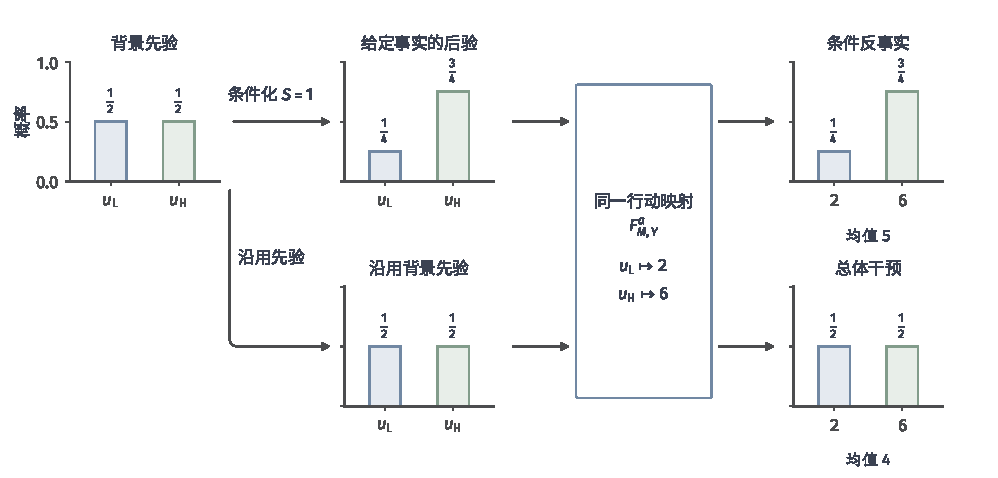
\includegraphics[width=169mm]{figures/01-mathematical-preliminaries/04-random-variables-distributions-and-causality/matplotlib/causal-two-point-pushforwards/figure.pdf}
  \caption{同一行动映射下的条件反事实与总体干预。背景$u_{\mathrm L},u_{\mathrm H}$的先验概率各为$1/2$，
  事实$S=1$将两者的后验概率更新为$1/4,3/4$；行动映射分别给出结果$2,6$。
  保留后验得到条件均值$5$，沿用先验得到总体干预均值$4$。
  概率柱使用共同的零基线与比例尺；溯因是给定模型内的条件化，不证明结构假设本身有效。}
  \label{fig:causal-abduction-intervention-prediction}
\end{figure*}
